\chapter{ПЕРЕНОС РЕЖИМНО-ЗАВИСИМОГО АППАРАТА НА РЕАЛЬНЫЕ ДАННЫЕ}
\label{chap:perenos-rezhimno-zavisimogo-apparata-na-realnye-dannye}

\section{Источники данных, ограничения и гипотезы эмпирической части}
\label{sec:istochniki-dannyh-ogranicheniya-i-gipotezy-empiricheskoi-chasti}

Эмпирическая часть работы опирается на два корпуса данных.

\subsection{Корпус 1: индексы промышленного производства}
\label{sec:korpus-1-indeksy-promyshlennogo-proizvodstva}

Файл ``февраль 2026 OKVED.XLS'' содержит 47 месячных рядов за период с января 2013 года по декабрь 2025 года, причём каждый ряд представлен в трёх версиях: скорректированной и сглаженной, скорректированной без сглаживания и сырой \cite{data-okved-xls}. Таблицы индексов промышленного производства подготовлены Владимиром Аркадьевичем Бессоновым и переданы автору через Ю.~А.~Полунина; методологический фон их построения сопоставим с официальной статистической практикой Росстата и публичным проектом НИУ ВШЭ по индексам интенсивности промышленного производства \cite{rosstat-ipp,hse-iipp}. В настоящей главе этот корпус используется как предварительная проверка переносимости метода, а не как основной объект эмпирического анализа.

\subsection{Корпус 2: выручка стабильных компаний}
\label{sec:korpus-2-vyruchka-stabilnyh-kompanii}

Файл ``Данные по выручке 2003--2022.xlsx'' содержит 23943 стабильные компании и годовой горизонт 2003--2022 годов \cite{data-revenue-xlsx}. Содержательный смысл этого корпуса связан не с отдельными фирмами как панелью, а с медианными траекториями групп и отраслей. Этот корпус является центральным для эмпирической части главы, поскольку лучше соответствует задаче анализа социально-экономических процессов на коротких окнах; его отраслевые ограничения далее рассматриваются с учётом официальных материалов по классификаторам \cite{minec-okved,rosstat-okved}. Подход к группам компаний согласуется с литературой по динамике фирм, где устойчивые различия в траекториях роста интерпретируются как различия в адаптации и стратегии компаний \cite{coad,polunin-2019,polunin-yudanov-2020}.

\subsection{Почему группы компаний экономически содержательны}
\label{sec:pochemu-gruppy-kompanii-ekonomicheski-soderzhatelny}

Разбиение компаний на группы по темпам роста 2010--2014 годов имеет не только технический, но и экономический смысл. Оно отражает различия в адаптации фирм к посткризисной перестройке среды: одна группа быстрее наращивает выручку, другая остаётся в более слабом положении, а промежуточная группа удерживает умеренную траекторию. Поэтому далее анализируются не абстрактные кластеры, а три типа медианной динамики типичной компании группы \cite{coad,polunin-2019,polunin-yudanov-2020}.

\subsection{Почему корпуса нельзя напрямую объединять}
\label{sec:pochemu-korpusa-nelzya-napryamuyu-obedinyat}

Индексы промышленного производства и выручка различаются по экономической природе, частоте наблюдений и отраслевой кодировке. Кроме того, переход между старыми кодами ОКВЭД и ОКВЭД2 не является полностью однозначным и требует специальных переходных ключей \cite{minec-okved,rosstat-okved}. Поэтому в основной части главы эти корпуса не сравниваются как единый массив. Индексы используются только как внешняя проверка переносимости режима анализа, тогда как содержательный эмпирический результат строится на выручке компаний.

\subsection{Ограничения данных}
\label{sec:ogranicheniya-dannyh}

Эмпирическая часть имеет четыре принципиальных ограничения, вытекающих как из природы самих рядов, так и из ограничений отраслевой классификации \cite{minec-okved,rosstat-okved}.

\begin{enumerate}
\def\labelenumi{\arabic{enumi}.}
\tightlist
\item
  На реальных данных невозможно точное восстановление истинной модели: исследование может опираться только на устойчивость результатов, повторяемость режимов и допустимость интерпретации.
\item
  Выручка и промышленные индексы имеют разную природу: сравнивать их уровни напрямую методологически неверно.
\item
  Около 22.2\% наблюдений по выручке не имеют отраслевого кода, поэтому отраслевой анализ требует предварительной фильтрации.
\item
  В работе сравниваются не уровни рядов, а режимы, интерпретируемость окна и допустимость выбранного контура чтения.
\end{enumerate}

\subsection{Гипотезы эмпирической части}
\label{sec:gipotezy-empiricheskoi-chasti}

В эмпирической части проверяются следующие гипотезы.

\begin{enumerate}
\def\labelenumi{\arabic{enumi}.}
\tightlist
\item
  Режимно-зависимый подход, построенный на синтетических данных, переносим на реальные данные по выручке как процедура выбора допустимого контура анализа.
\item
  Полные интервалы по выручке чаще дают высокое качество подгонки, но реже допускают содержательное чтение, чем короткие окна.
\item
  Группы и отрасли по выручке различаются не только формой траектории, но и типом допустимой интерпретации.
\item
  Промышленные индексы могут использоваться как внешняя проверка переносимости метода, но не как второй равноправный центр главы.
\end{enumerate}

\section{Дизайн эмпирической части}
\label{sec:dizain-empiricheskoi-chasti}

В бакалаврской версии работы эмпирическая глава организована вокруг одного основного вопроса: переносится ли режимно-зависимый подход из синтетической части на реальные данные по выручке. Постановка этого вопроса опирается на различие между контролируемым синтетическим экспериментом и реальными статистическими корпусами, зафиксированное в литературе по нелинейной динамике, регрессионному анализу и эконометрике временных рядов \cite{strogatz,montgomery,hamilton,box-jenkins}.

Для ответа на этот вопрос использовались три последовательных шага.

\begin{enumerate}
\def\labelenumi{\arabic{enumi}.}
\tightlist
\item
  Сначала на промышленном корпусе выполнялась краткая внешняя проверка переносимости построенного маршрута анализа.
\item
  Затем на выручке компаний исследовались медианные траектории трёх групп фирм, различающихся по темпам роста.
\item
  После этого анализ переносился на отраслевой подкорпус выручки, где проверялась читаемость коротких окон уже на уровне секторов.
\end{enumerate}

Таким образом, в основной текст вынесена прежде всего денежная линия исследования, тогда как промышленный корпус выполняет роль предварительной проверки устойчивости метода вне синтетической среды.

\section{Предварительная проверка переносимости на промышленных индексах}
\label{sec:predvaritelnaya-proverka-perenosimosti-na-promyshlennyh-indeksah}

\subsection{Вопрос, данные и главный результат}
\label{sec:vopros-dannye-i-glavnyi-rezultat}

Вопрос этого шага состоял в том, сохраняется ли построенный в главе 2 маршрут анализа на реальных месячных рядах. Для этого сравнивались три версии одного и того же промышленного процесса: скорректированная и сглаженная, скорректированная без сглаживания и сырая.

Главный результат здесь формулируется достаточно чётко. В качестве рабочего слоя наблюдения был выбран скорректированный, но не сглаженный ряд. Сглаженный ряд создавал избыточную упорядоченность, а сырой --- избыточную турбулентность. На выбранном слое было показано, что короткое окно и на реальных данных не должно читаться автоматически: сначала определяется режим, затем проверяется интерпретируемость, и только после этого допускается регрессионный контур. Этот шаг важен и как защитная проверка, поскольку показывает, что построенная процедура не является артефактом только денежного корпуса.

\subsection{Ограничение этого шага}
\label{sec:ogranichenie-etogo-shaga}

Промышленный корпус не является центральным эмпирическим результатом главы. Его функция ограничена предварительной проверкой переносимости метода. Подробные отраслевые карточки и промежуточные карты в основной текст не включаются, поскольку содержательный центр эмпирической части расположен в анализе выручки.

Расширенные карточки отраслей и полные сводки по промышленному корпусу приведены в приложениях.

\section{Группы компаний по выручке}
\label{sec:gruppy-kompanii-po-vyruchke}

\subsection{Вопрос и данные}
\label{sec:vopros-i-dannye}

Основной эмпирический вопрос главы формулируется так: переносится ли режимно-зависимый подход на реальные годовые траектории выручки. Для ответа на него компании были разделены на три группы по темпам роста 2010--2014 годов: группу высоких темпов роста, группу низких темпов роста и группу средних темпов роста. В каждой группе оказалось по 2394 фирмы.

\subsection{Режимное чтение}
\label{sec:rezhimnoe-chtenie}

На полных интервалах 2014--2019 и 2014--2022 годов было показано, что высокое качество подгонки ещё не означает содержательной читаемости. Большинство полных интервалов у групп выручки относится к низкодисперсионным окнам, где регрессия формально может выглядеть устойчивой, но не даёт надёжной структурной интерпретации. Короткие окна длины 5 и 7 лет оказываются информативнее: именно на них различаются допустимые режимы чтения для групп высоких, низких и средних темпов роста.

Чтобы не сохранять служебные метки без пояснения, в дальнейшем используются следующие русские формулировки. Структурно читаемым называется такое окно, в котором дисперсия темпа прироста не вырождается, регрессоры не схлопываются в тяжёлую коллинеарность, а оценённые коэффициенты допускают содержательное чтение. Если окно не допускает содержательной интерпретации, это означает, что коэффициенты не должны использоваться как аргумент о памяти, инерции или устойчивом законе движения. Если окно требует фазового чтения, то допустимо говорить только о форме траектории, локальном переломе и характере перехода между режимами, но не о надёжной лаговой структуре. Формула вида «полный интервал остаётся интерпретируемым» в настоящей главе означает только то, что рассматриваемый интервал не переходит автоматически в режим отказа от интерпретации; она не означает, что единая регрессионная спецификация одинаково пригодна для всех вложенных подокон.

\subsection{Главный результат}
\label{sec:glavnyi-rezultat}

Главный результат первого блока по выручке состоит в том, что группы фирм различаются не только уровнем и направлением роста, но и типом допустимого анализа. Группа высоких темпов роста чаще открывается для интерпретации на коротких окнах, группа низких темпов роста чаще остаётся закрытой для содержательного регрессионного чтения, а группа средних темпов роста занимает промежуточное положение. Следовательно, режимно-зависимый подход переносится на реальные годовые ряды выручки и позволяет различать не только траектории, но и саму возможность их анализа.

На рисунке~\ref{fig:b1-trajectories} показано, что различие между тремя группами выражается не в одном агрегированном коэффициенте, а в форме самих траекторий.

\begin{figure}[htbp]
\centering
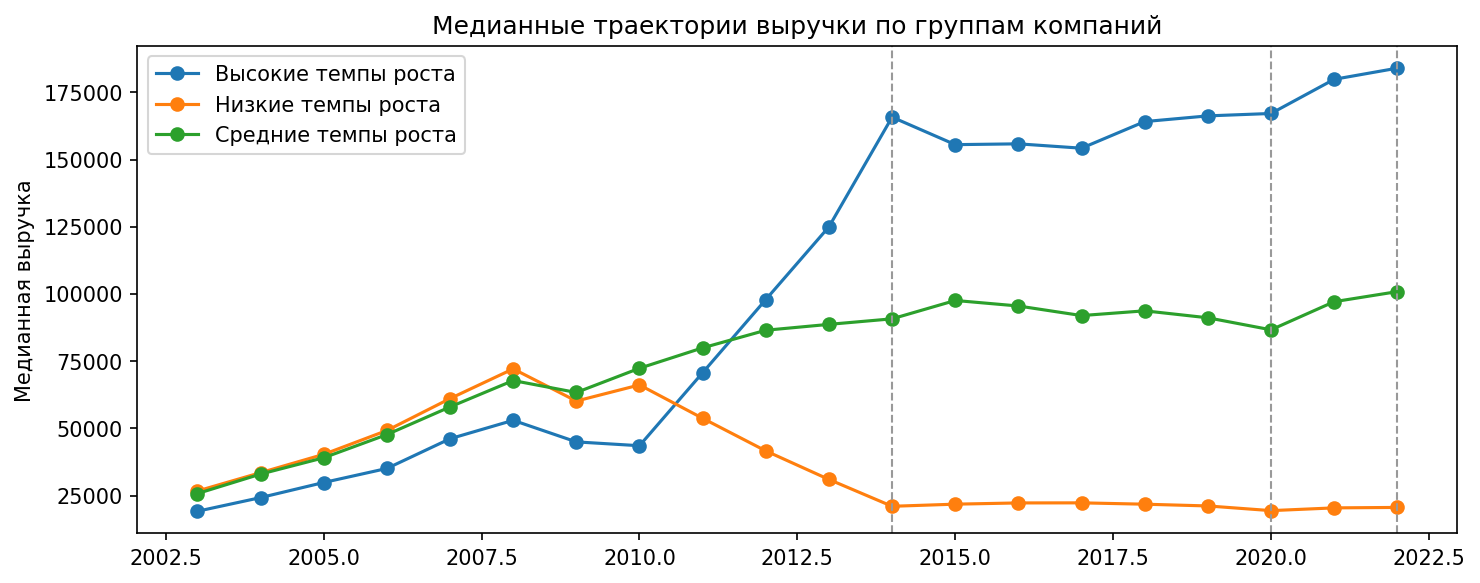
\includegraphics[width=\linewidth,keepaspectratio]{outputs/real_data/revenue_b1/group_trajectories.png}
\caption{Медианные траектории выручки трёх групп компаний\\ \textit{Источник: расчёты автора по данным корпуса ``Данные по выручке 2003--2022.xlsx''.}}
\label{fig:b1-trajectories}
\end{figure}

На рисунке~\ref{fig:b1-interpretable} показано уже другое свойство тех же групп: они различаются именно по доле окон, допускающих содержательное чтение короткого окна.

\begin{figure}[htbp]
\centering
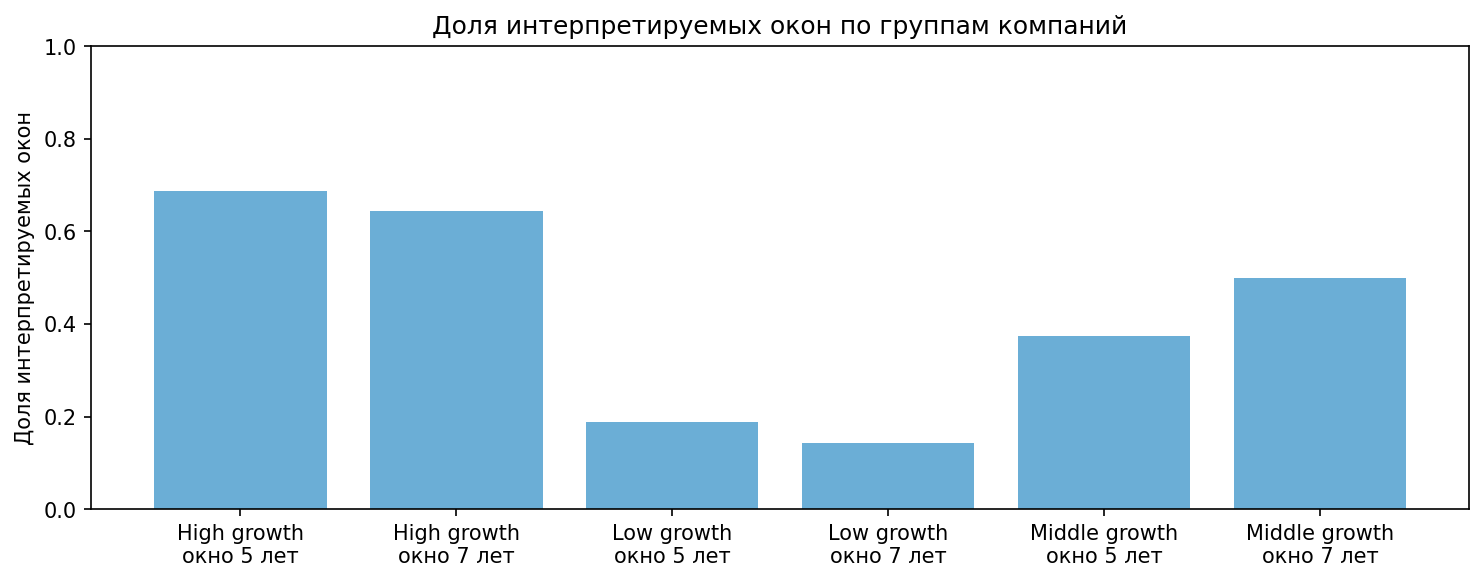
\includegraphics[width=\linewidth,keepaspectratio]{outputs/real_data/revenue_b1/window_interpretable_share.png}
\caption{Доля коротких окон, допускающих содержательную интерпретацию, по группам компаний\\ \textit{Источник: расчёты автора по данным корпуса ``Данные по выручке 2003--2022.xlsx''.}}
\label{fig:b1-interpretable}
\end{figure}

\subsection{Экономический смысл различий между группами}
\label{sec:ekonomicheskii-smysl-razlichii-mezhdu-gruppami}

Методологический результат этого блока сводится к различию допустимых контуров чтения, но сами различия между группами имеют и экономический смысл. Краткая сводка приведена в таблице~\ref{tab:b1-groups-economic-meaning}.

\begin{table}[htbp]
\centering
\caption{Группы компаний по выручке: режимное чтение и экономический смысл}
\label{tab:b1-groups-economic-meaning}
\begin{tabular}{p{0.2\linewidth}p{0.22\linewidth}p{0.23\linewidth}p{0.25\linewidth}}
\toprule
Группа & Доминирующее чтение & Интерпретируемая доля окон & Осторожная экономическая интерпретация \\
\midrule
Высокие темпы роста & структурное на \(W=5\), фазовое на \(W=7\) & 0.6875 и 0.6429 & группа быстрее адаптируется к изменениям среды и чаще сохраняет читаемую локальную динамику \\
Низкие темпы роста & окно чаще не допускает содержательной интерпретации & 0.1875 и 0.1429 & группа дольше остаётся в инерционном или низкодисперсионном режиме, где локальная регрессия малоинформативна \\
Средние темпы роста & промежуточный режим, на \(W=7\) чаще структурное чтение & 0.3750 и 0.5000 & группа занимает промежуточное положение: динамика менее закрыта, чем у аутсайдеров, но менее устойчива к чтению, чем у лидеров \\
\bottomrule
\end{tabular}
\end{table}

Эта таблица нужна для аккуратного перевода режима анализа в язык фирменной динамики, а не для причинного объяснения роста. Высокая группа соответствует компаниям, которые успешнее адаптируются к изменениям среды; низкая --- фирмам с затруднённым восстановлением; средняя фиксирует промежуточный сценарий. Такая трактовка согласуется с логикой работ о посткризисной адаптации российских компаний и о различии устойчивых типов фирменного роста \cite{polunin-yudanov-2020,medovnikov,baranova-yudanov}. Различие групп состоит, таким образом, не только в уровне медианной выручки, но и в степени допустимости содержательного чтения короткого окна.

\subsection{Ограничение}
\label{sec:ogranichenie}

Этот результат относится к группам фирм, агрегированным по прошлому темпу роста. Поэтому он не описывает ещё отраслевые различия и не даёт оснований переносить выводы на всю денежную реальность без дополнительной проверки по секторам.

\section{Отраслевой подкорпус выручки}
\label{sec:otraslevoi-podkorpus-vyruchki}

\subsection{Формирование корпуса}
\label{sec:formirovanie-korpusa}

Если первый блок работал с группами фирм по темпам роста, то второй блок переводит линию выручки на отраслевой уровень. Единицей анализа становится двухзначный сектор старого ОКВЭД.

Во втором блоке использовался жёсткий фильтр:

\begin{itemize}
\tightlist
\item
  заполненный и нормализуемый код;
\item
  устойчивое присутствие в годовой панели;
\item
  не менее 100 фирм в секторе.
\end{itemize}

После фильтра получен основной отраслевой слой (таблица~\ref{tab:sector-filter}).

\begin{center}
\captionof{table}{Результат отбора отраслевого подкорпуса выручки}
\label{tab:sector-filter}
\end{center}

{\def\LTcaptype{none} % do not increment counter
\begin{longtable}[]{@{}rrrr@{}}
\toprule\noalign{}
total firms & firms with OKVED & included firms & included sectors \\
\midrule\noalign{}
\endhead
\bottomrule\noalign{}
\endlastfoot
23943 & 18628 & 17497 & 29 \\
\end{longtable}
}

Линия выручки здесь упирается не только в моделирование, но и в качество кодировки. Найденный компромисс позволил сохранить и масштаб, и интерпретируемость. Благодаря этому отраслевой блок стал самостоятельной линией анализа, а не приложением к групповому блоку.

\subsection{Полные интервалы и короткие окна}
\label{sec:polnye-intervaly-i-korotkie-okna}

На полном интервале отраслевой блок оказался менее закрытым, чем групповой; сводные результаты приведены в таблице~\ref{tab:sector-full-intervals}.

\begin{center}
\captionof{table}{Допустимые контуры чтения на полных интервалах отраслевой выручки}
\label{tab:sector-full-intervals}
\end{center}

{\def\LTcaptype{none} % do not increment counter
\begin{longtable}[]{@{}
  >{\raggedright\arraybackslash}p{(\linewidth - 8\tabcolsep) * \real{0.1579}}
  >{\raggedleft\arraybackslash}p{(\linewidth - 8\tabcolsep) * \real{0.2105}}
  >{\raggedleft\arraybackslash}p{(\linewidth - 8\tabcolsep) * \real{0.2105}}
  >{\raggedleft\arraybackslash}p{(\linewidth - 8\tabcolsep) * \real{0.2105}}
  >{\raggedleft\arraybackslash}p{(\linewidth - 8\tabcolsep) * \real{0.2105}}@{}}
\toprule\noalign{}
\begin{minipage}[b]{\linewidth}\raggedright
Интервал
\end{minipage} & \begin{minipage}[b]{\linewidth}\raggedleft
структурное чтение
\end{minipage} & \begin{minipage}[b]{\linewidth}\raggedleft
фазовое чтение
\end{minipage} & \begin{minipage}[b]{\linewidth}\raggedleft
агрегированный регрессионный контур
\end{minipage} & \begin{minipage}[b]{\linewidth}\raggedleft
окно не допускает содержательной интерпретации
\end{minipage} \\
\midrule\noalign{}
\endhead
\bottomrule\noalign{}
\endlastfoot
2014--2019 & 15 & 1 & 2 & 11 \\
2014--2022 & 20 & 4 & 1 & 4 \\
\end{longtable}
}

Содержательный смысл этого результата состоит в различии двух типов агрегации: группы фирм по прошлому темпу роста смешивают разные механизмы внутри общего роста, тогда как отрасли чаще объединяют фирмы с более близкой экономической логикой. Поэтому отраслевой денежный слой оказался более читаемым на полном интервале.

Именно на коротких окнах длины 5 и 7 лет отраслевой блок превратился в полноценную карту читаемости. Важно, что эта карта показывает не просто различие форм рядов, а различие аналитической доступности отраслей: где короткое окно допускает содержательное чтение, а где не допускает его даже при формально приемлемой подгонке. При длине окна 7 наиболее читаемыми оказались:

\begin{itemize}
\tightlist
\item
  производство строительных металлических конструкций, производство мебели для офисов и предприятий торговли, а также хранение и складирование зерна с долей интерпретируемых окон 0.9286;
\item
  производство изделий из бетона для строительства, автомобильные грузовые перевозки, разработка программного обеспечения, производство машин для пищевой промышленности, обслуживание электрооборудования, производство фармацевтических изделий и производство гофрированного картона и тары с долей интерпретируемых окон 0.8571.
\end{itemize}

Наиболее закрытыми оказались:

\begin{itemize}
\tightlist
\item
  розничная торговля в неспециализированных магазинах преимущественно пищевыми продуктами с нулевой долей интерпретируемых окон;
\item
  сдача внаём собственного нежилого недвижимого имущества, распределение воды, организация похорон и некоторые другие сектора, где окно чаще не допускает содержательной интерпретации.
\end{itemize}

Следовательно, второй блок дал уже не общий анализ групп, а именно отраслевую карту читаемости выручки.

Рисунок~\ref{fig:b2-fit} важно понимать не как витрину лучших значений \(R^2\). Его задача состоит только в демонстрации неоднородности полного интервала: даже высокое качество подгонки само по себе не означает структурной читаемости. В этом смысле рисунок выступает негативным контролем для слишком прямого чтения отраслевых траекторий.

\begin{figure}[htbp]
\centering
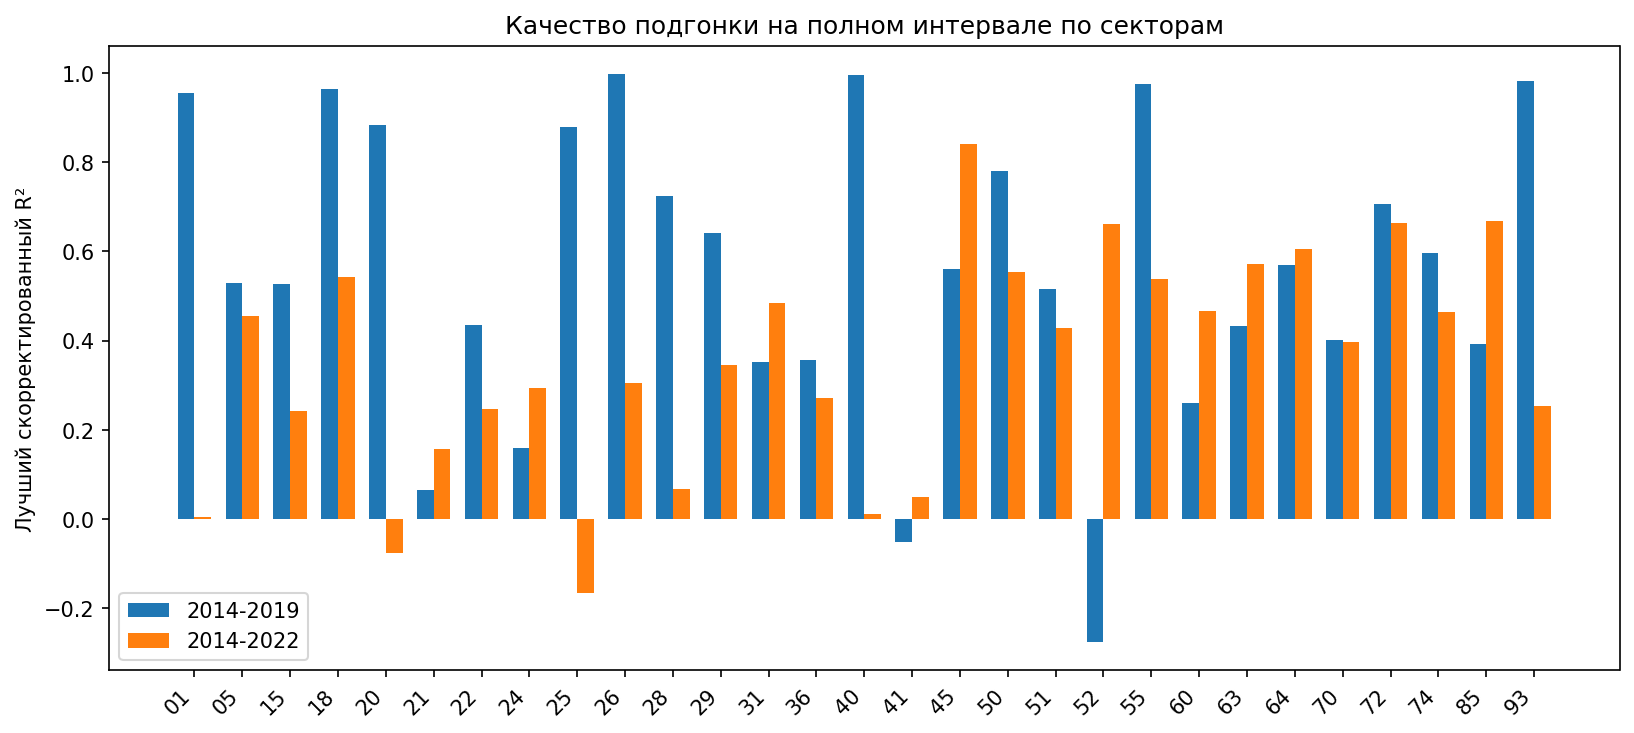
\includegraphics[width=\linewidth,keepaspectratio]{outputs/real_data/revenue_b2/sector_interval_best_fit.png}
\caption{Качество подгонки на полном интервале по отраслевым траекториям выручки\\ \textit{Источник: расчёты автора по данным корпуса ``Данные по выручке 2003--2022.xlsx'' после отраслевой фильтрации.}}
\label{fig:b2-fit}
\end{figure}

Рисунок~\ref{fig:b2-interpretable} является центральной иллюстрацией всего отраслевого блока, поскольку именно он показывает различия между секторами по допустимости чтения короткого окна. Здесь расположен главный позитивный результат этой части главы: карта аналитической доступности отраслевых денежных рядов.

\begin{figure}[htbp]
\centering
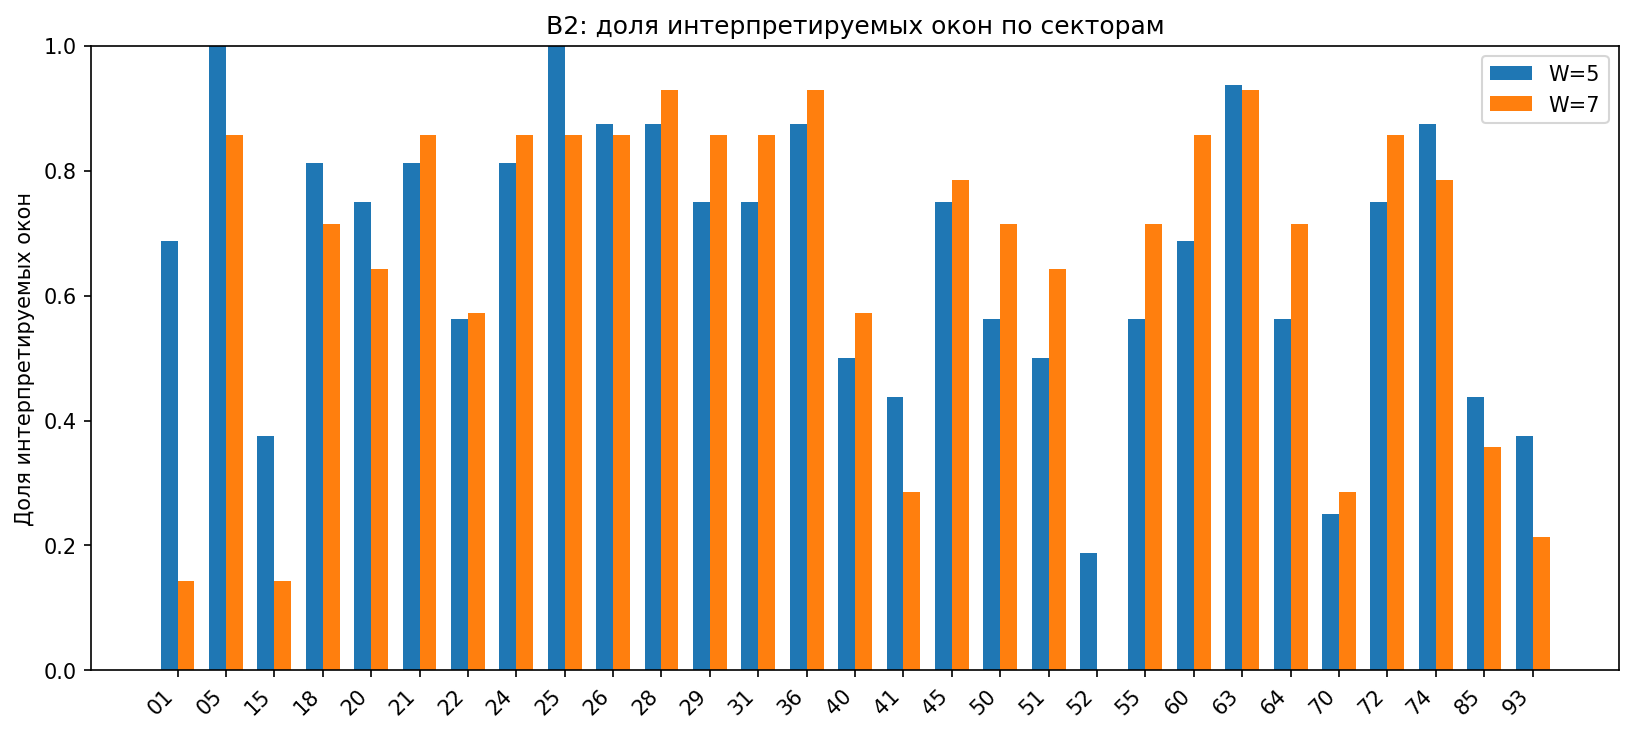
\includegraphics[width=\linewidth,keepaspectratio]{outputs/real_data/revenue_b2/sector_interpretable_share.png}
\caption{Доля интерпретируемых коротких окон по отраслевым траекториям выручки\\ \textit{Источник: расчёты автора по данным корпуса ``Данные по выручке 2003--2022.xlsx'' после отраслевой фильтрации.}}
\label{fig:b2-interpretable}
\end{figure}

Именно второй блок переводит денежную линию из первичной эмпирической проверки в самостоятельный прикладной корпус. Здесь линия выручки становится самостоятельной отраслевой картой допустимого и недопустимого чтения короткого окна.

\subsection{Три мини-кейса отраслевой выручки}
\label{sec:tri-mini-keisa-otraslevoi-vyruchki}

Чтобы отраслевой блок не оставался только картой режимных меток, далее рассматриваются три сектора, выбранные как характерные точки отраслевой карты читаемости.

Прямые расчётные различия между этими секторами удобно зафиксировать ещё до их качественной интерпретации. Рисунок~\ref{fig:sector-minicases-overview} строится в двух слоях: слева представлены индексированные траектории медианной выручки, справа --- поведение поздних окон \(W=7\). Правая колонка имеет самостоятельную методологическую нагрузку: она показывает, что сектор 63 почти полностью сохраняет структурную читаемость, сектор 29 остаётся интерпретируемым, но демонстрирует большую чувствительность к локальному сдвигу окна, тогда как сектор 52 систематически переводится в режим отказа от содержательной регрессии. Следовательно, различие между секторами фиксируется не только описательно, но и как различие допустимых контуров анализа.

\begin{figure}[htbp]
\centering
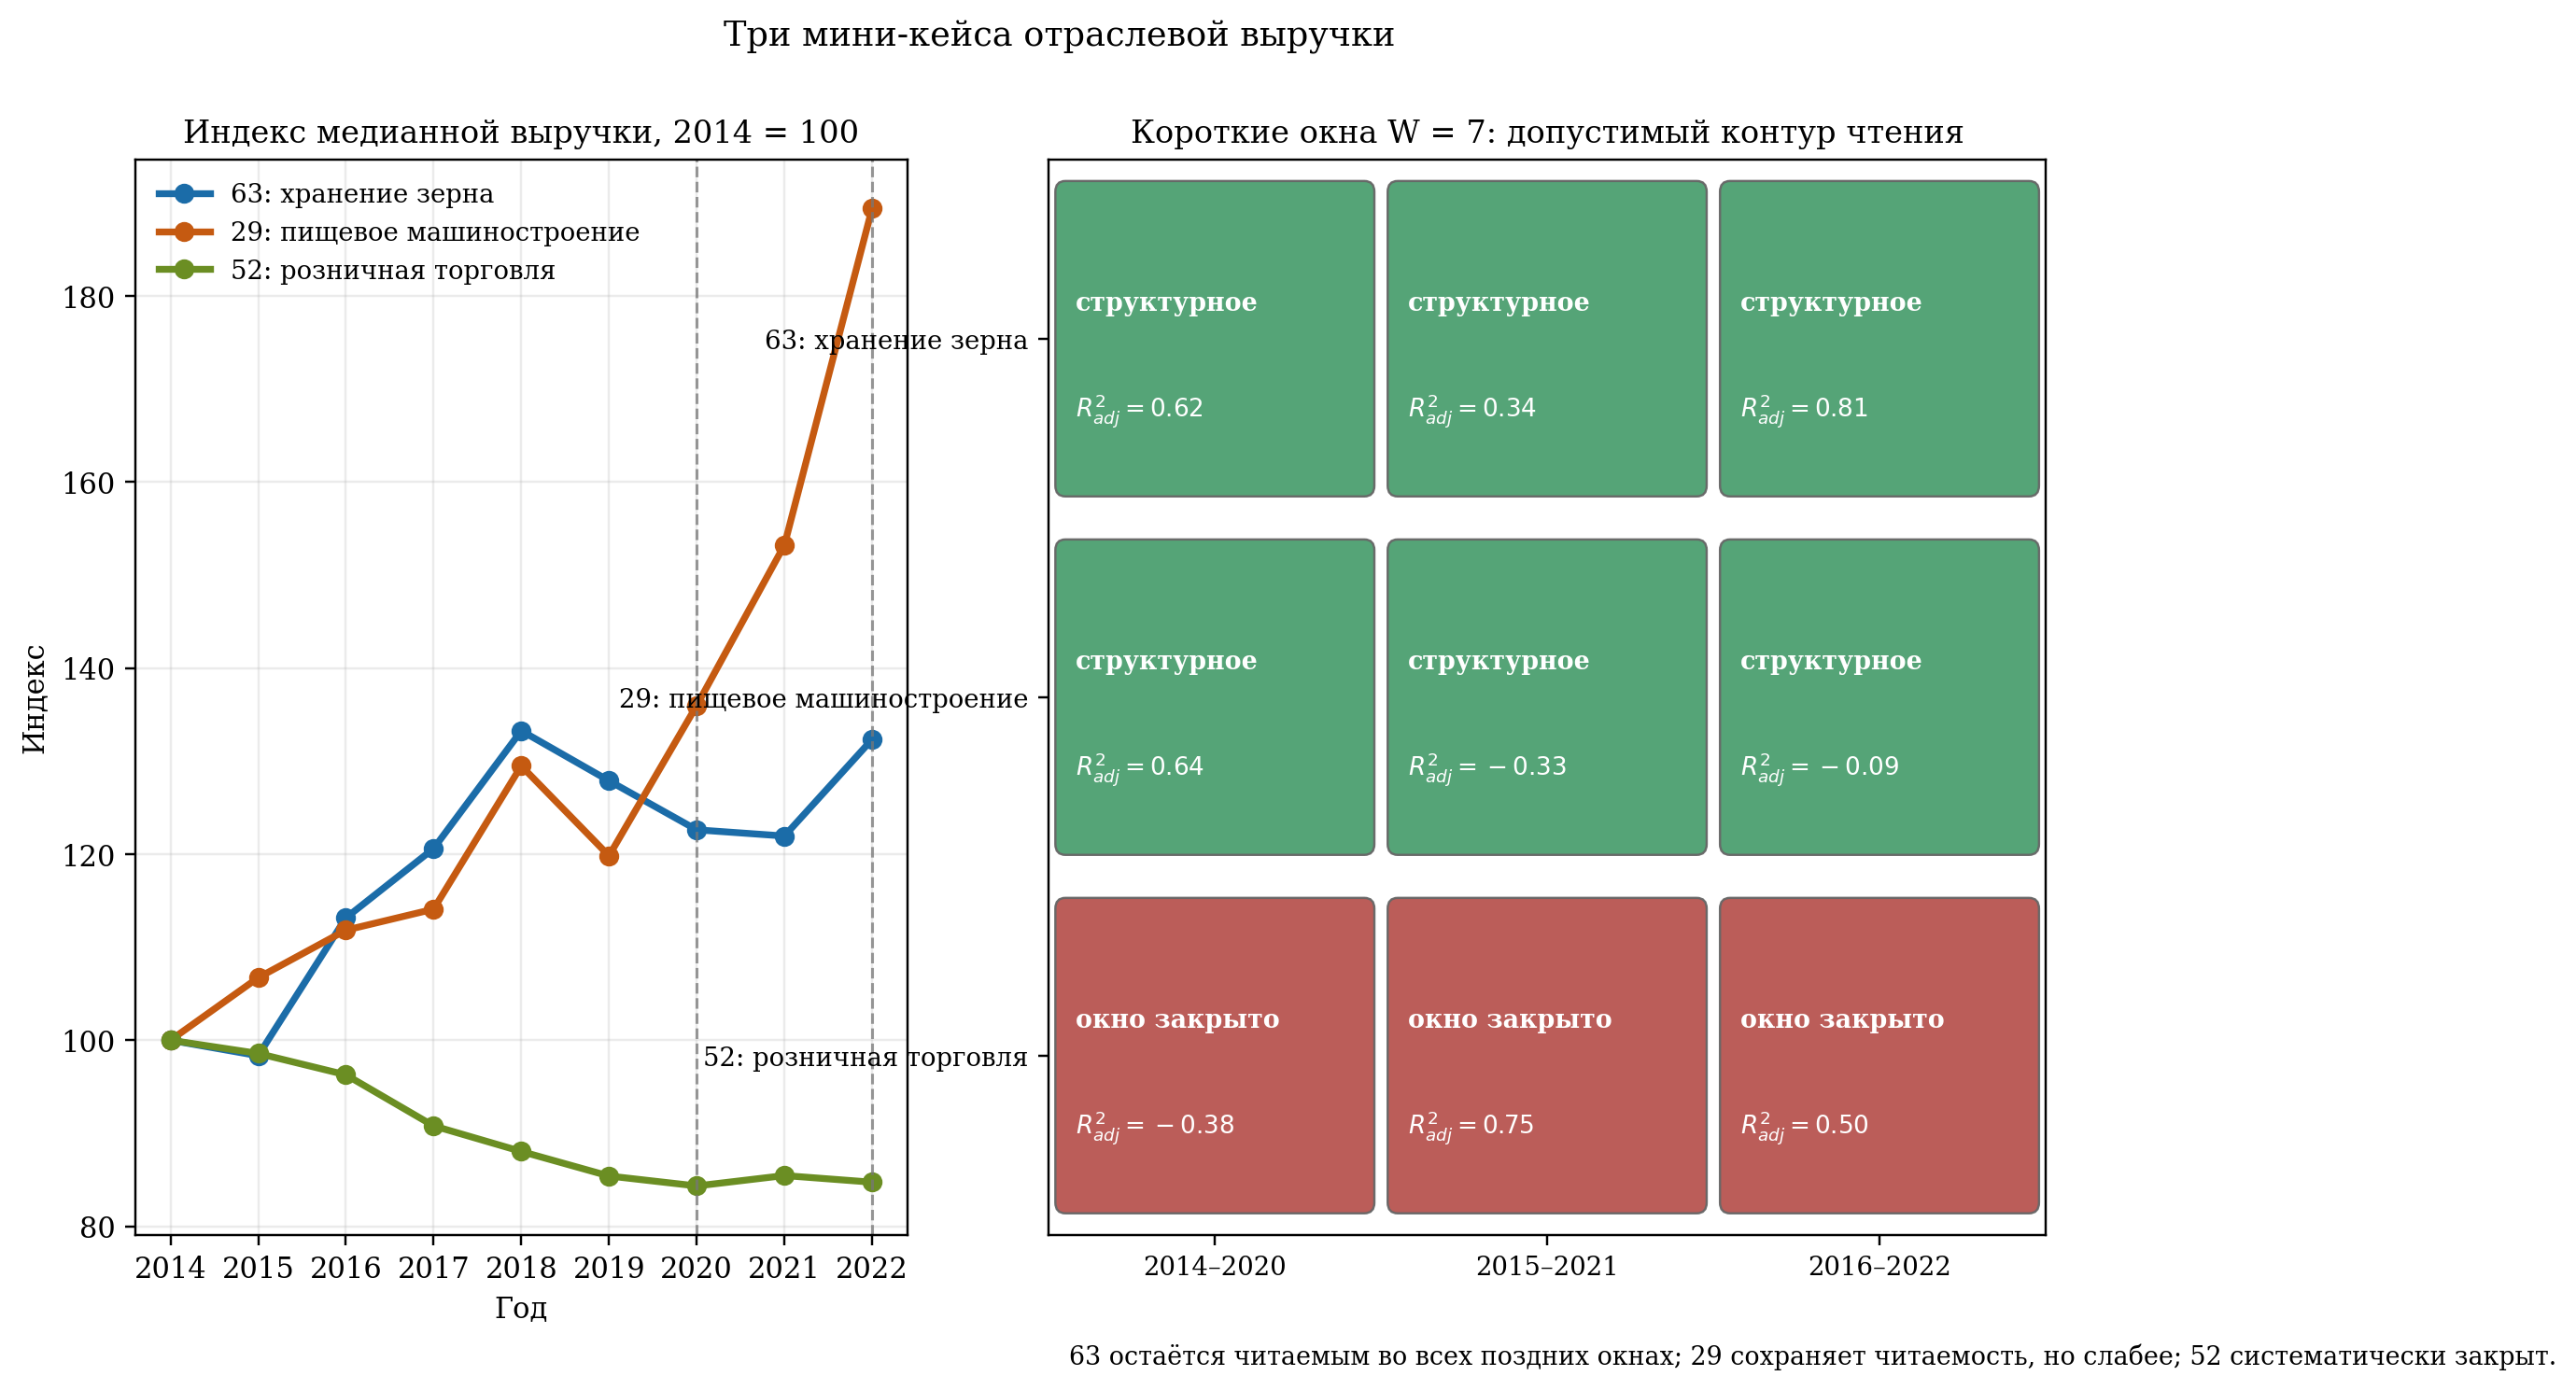
\includegraphics[width=0.96\textwidth]{../outputs/real_data/revenue_b2/sector_minicases_overview.png}
\caption{Три мини-кейса отраслевой выручки: траектории и читаемость короткого окна\\ \textit{Источник: расчёты автора по данным корпуса ``Данные по выручке 2003--2022.xlsx'' после отраслевой фильтрации.}}
\label{fig:sector-minicases-overview}
\end{figure}

\textbf{1. Сектор 63 --- хранение и складирование зерна.} При \(W=7\) доля интерпретируемых окон достигает 0.9286, а доминирующий контур остаётся структурным. Медианная траектория сектора демонстрирует умеренно возрастающую динамику без устойчивого перехода в низкодисперсионный режим. На поздних окнах ряд сохраняет аналитическую доступность и лишь эпизодически требует более осторожного фазового чтения. Следовательно, данный сектор систематически допускает содержательное локальное чтение. Вместе с тем из этого не следует, что полный интервал можно трактовать как единую устойчивую лаговую модель или что выявленный режим раскрывает причины роста сектора.

\textbf{2. Сектор 29 --- производство машин и оборудования для изготовления пищевых продуктов, включая напитки, и табачных изделий.} Этот сектор входит в число лидеров по читаемости (\(0.8571\) при \(W=7\)), однако его динамика существенно менее инерционна, чем у сектора 63. На траектории заметны переломы 2020 и 2022 годов, а поздние окна уже не сводятся к однотипному поведению. Тем не менее сектор не утрачивает аналитической доступности: структурное чтение здесь сохраняется, но сочетается с повышенной чувствительностью к режимному сдвигу. Следовательно, отрасль допускает содержательный анализ даже при выраженных шоковых эпизодах. В то же время наличие структурно читаемых окон не означает, что вся траектория на полном интервале является однородной и допускает единое регрессионное описание.

\textbf{3. Сектор 52 --- розничная торговля в неспециализированных магазинах преимущественно пищевыми продуктами, включая напитки, и табачными изделиями.} При \(W=7\) доля интерпретируемых окон равна нулю, а доминирует низкодисперсионный режим с отказом от содержательной регрессии. Внешне траектория выглядит устойчивой, однако именно эта сглаженность делает короткое окно аналитически бедным. На локальном уровне регрессионный контур почти не даёт надёжной структурной информации. Следовательно, в выбранной нормировке сектор оказывается методологически закрытым для содержательного чтения короткого окна. Из этого, однако, не следует, что в секторе отсутствует экономическая динамика; вывод касается только границ интерпретации данного ряда.

\subsubsection{Три фирменных якоря внутри отраслевых кейсов}
\label{sec:tri-firmennyh-yakorya-vnutri-otraslevyh-keisov}

Чтобы отраслевой результат не оставался полностью обезличенным, целесообразно показать и три фирменных якоря внутри уже отобранных секторов. В качестве таких якорей выбраны ОАО «Еланский элеватор» для сектора 63, АО «ТЭСМО» для сектора 29 и Шестихинское потребительское общество для сектора 52. Эти фирмы не интерпретируются как статистические представители всего сектора; их задача скромнее --- показать, каким образом медианная логика сектора может соотноситься с конкретной хозяйственной траекторией.

\begin{figure}[htbp]
\centering
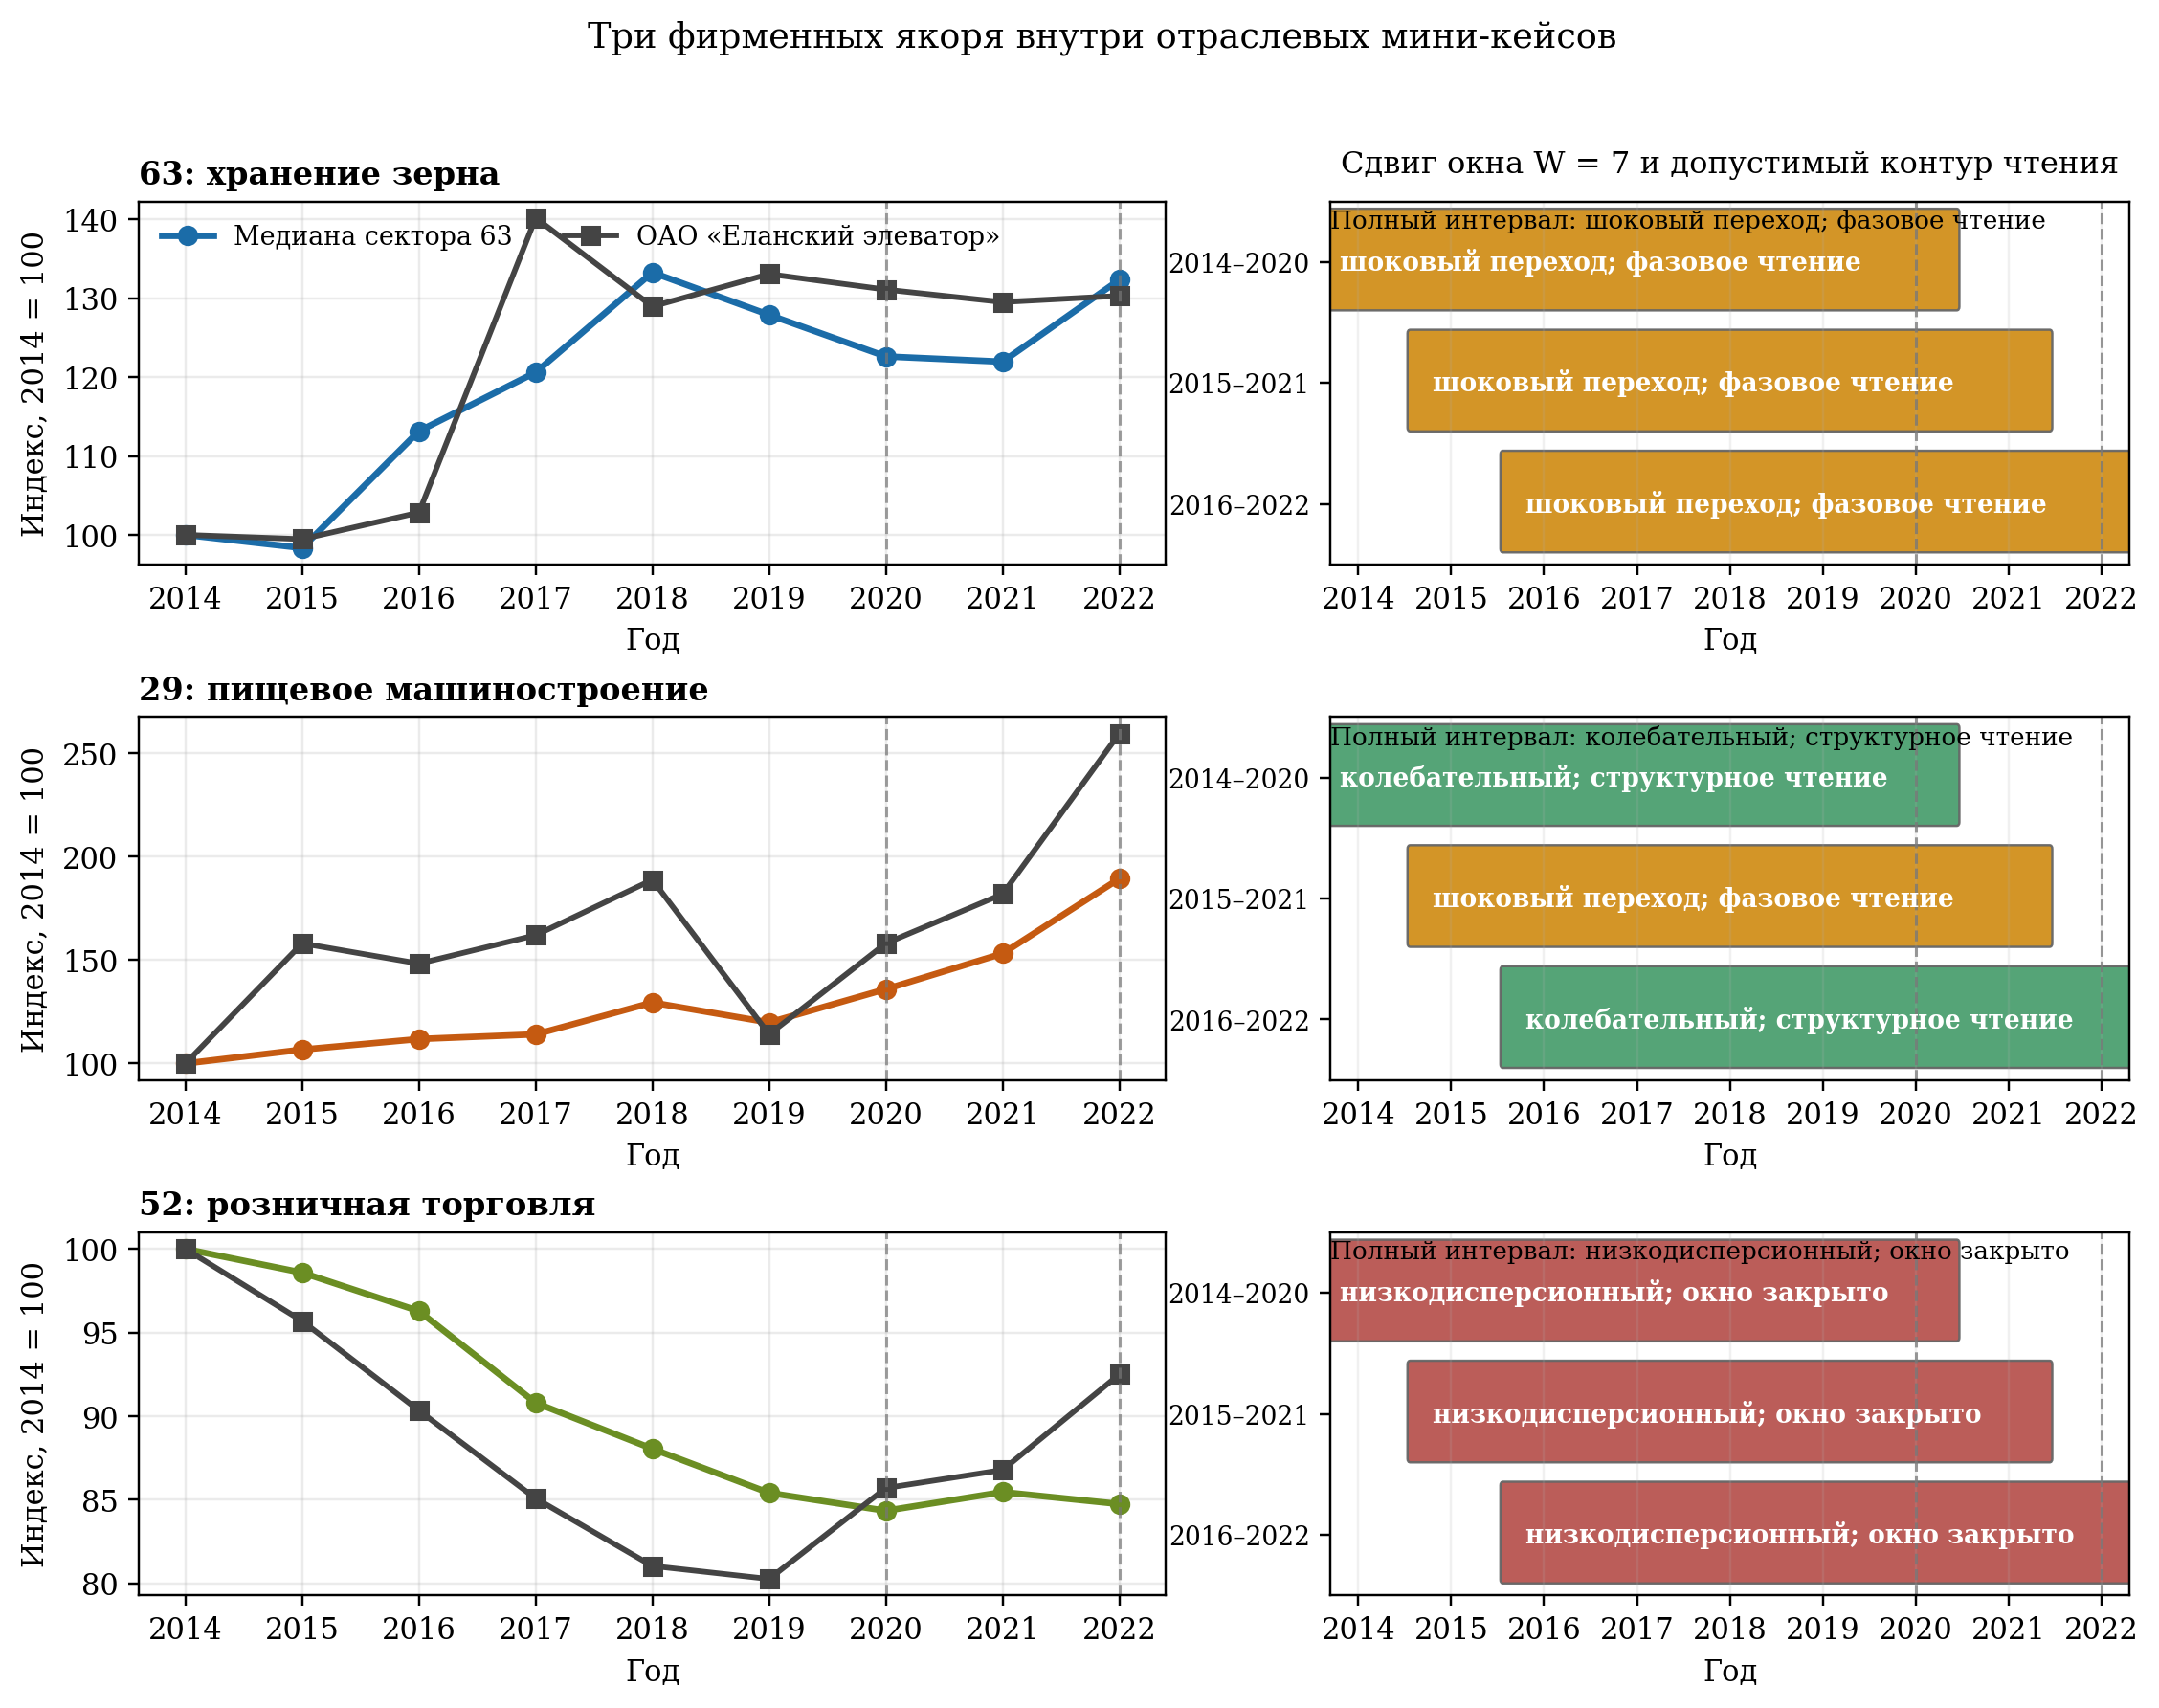
\includegraphics[width=0.98\textwidth]{../outputs/real_data/revenue_b2/company_case_anchors.png}
\caption{Три фирменных якоря внутри отраслевых мини-кейсов\\ \textit{Источник: расчёты автора по данным корпуса ``Данные по выручке 2003--2022.xlsx'' после отраслевой фильтрации.}}
\label{fig:company-case-anchors}
\end{figure}

Рисунок~\ref{fig:company-case-anchors} вводится не для замены медианных отраслевых траекторий отдельными фирмами, а для проверки того, воспроизводится ли на уровне конкретной компании тот же порядок анализа, который был выработан в главе~2: сначала режим, затем интерпретируемость окна, затем допустимый контур чтения. По сектору 63 этот рисунок даёт важную оговорку: фирма из зернового хранения оказывается более шоково-чувствительной, чем медиана сектора, и на всех поздних окнах \(W=7\) требует фазового чтения. Следовательно, даже внутри хорошо читаемого сектора отдельная компания может быть более турбулентной, чем агрегированный ряд.

По сектору 29, напротив, фирменный якорь хорошо поддерживает отраслевой результат. Для АО «ТЭСМО» полный интервал сохраняет интерпретируемость, а при сдвиге окна возникает именно тот режимный переход, который и делает сектор содержательно интересным: структурное чтение на окне 2014--2020 годов, фазовое --- на окне 2015--2021 годов и возврат к структурному чтению на окне 2016--2022 годов. Здесь связь с аппаратом главы~2 прямая: на фирме воспроизводится та же логика переключения контуров, что и на синтетических рядах и на медианной траектории сектора.

По сектору 52 фирменный якорь подтверждает противоположный случай. Шестихинское потребительское общество воспроизводит общий низкодисперсионный профиль сектора: полный интервал и все поздние окна \(W=7\) остаются закрытыми для содержательной регрессии. Это наблюдение принципиально важно, поскольку показывает, что сектор 52 закрыт не только как обезличенный агрегат, но и на уровне конкретной фирмы близкого масштаба.

Следовательно, фирменные якоря не заменяют отраслевой анализ, но придают ему предметную опору. Они показывают, что карта отраслевой читаемости относится не к абстрактным линиям, а к реальным хозяйственным траекториям: в одних секторах даже фирменный уровень допускает осмысленное короткое чтение, в других --- требует фазовой осторожности, а в третьих остаётся методологически закрытым.

\subsection{Шоки 2020 и 2022}
\label{sec:shoki-2020-i-2022}

Шоки 2020 и 2022 годов представляют интерес не только как внешние разрывы траектории, но и как проверка устойчивости уже найденного аналитического контура. В данном разделе рассматривается не столько амплитуда самого шока, сколько перестройка режима чтения ряда. Для 2020 года сравниваются последнее предшоковое окно 2013--2019 годов и первое окно, содержащее шок, 2014--2020 годов. Для 2022 года, ввиду окончания наблюдений, сравниваются предшоковое окно 2015--2021 годов и первое окно, включающее 2022 год, 2016--2022 годов. Соответствие кодов и названий секторов, упоминаемых далее, вынесено в приложение~\ref{app:sector-code-name-map}.

\begin{figure}[htbp]
\centering
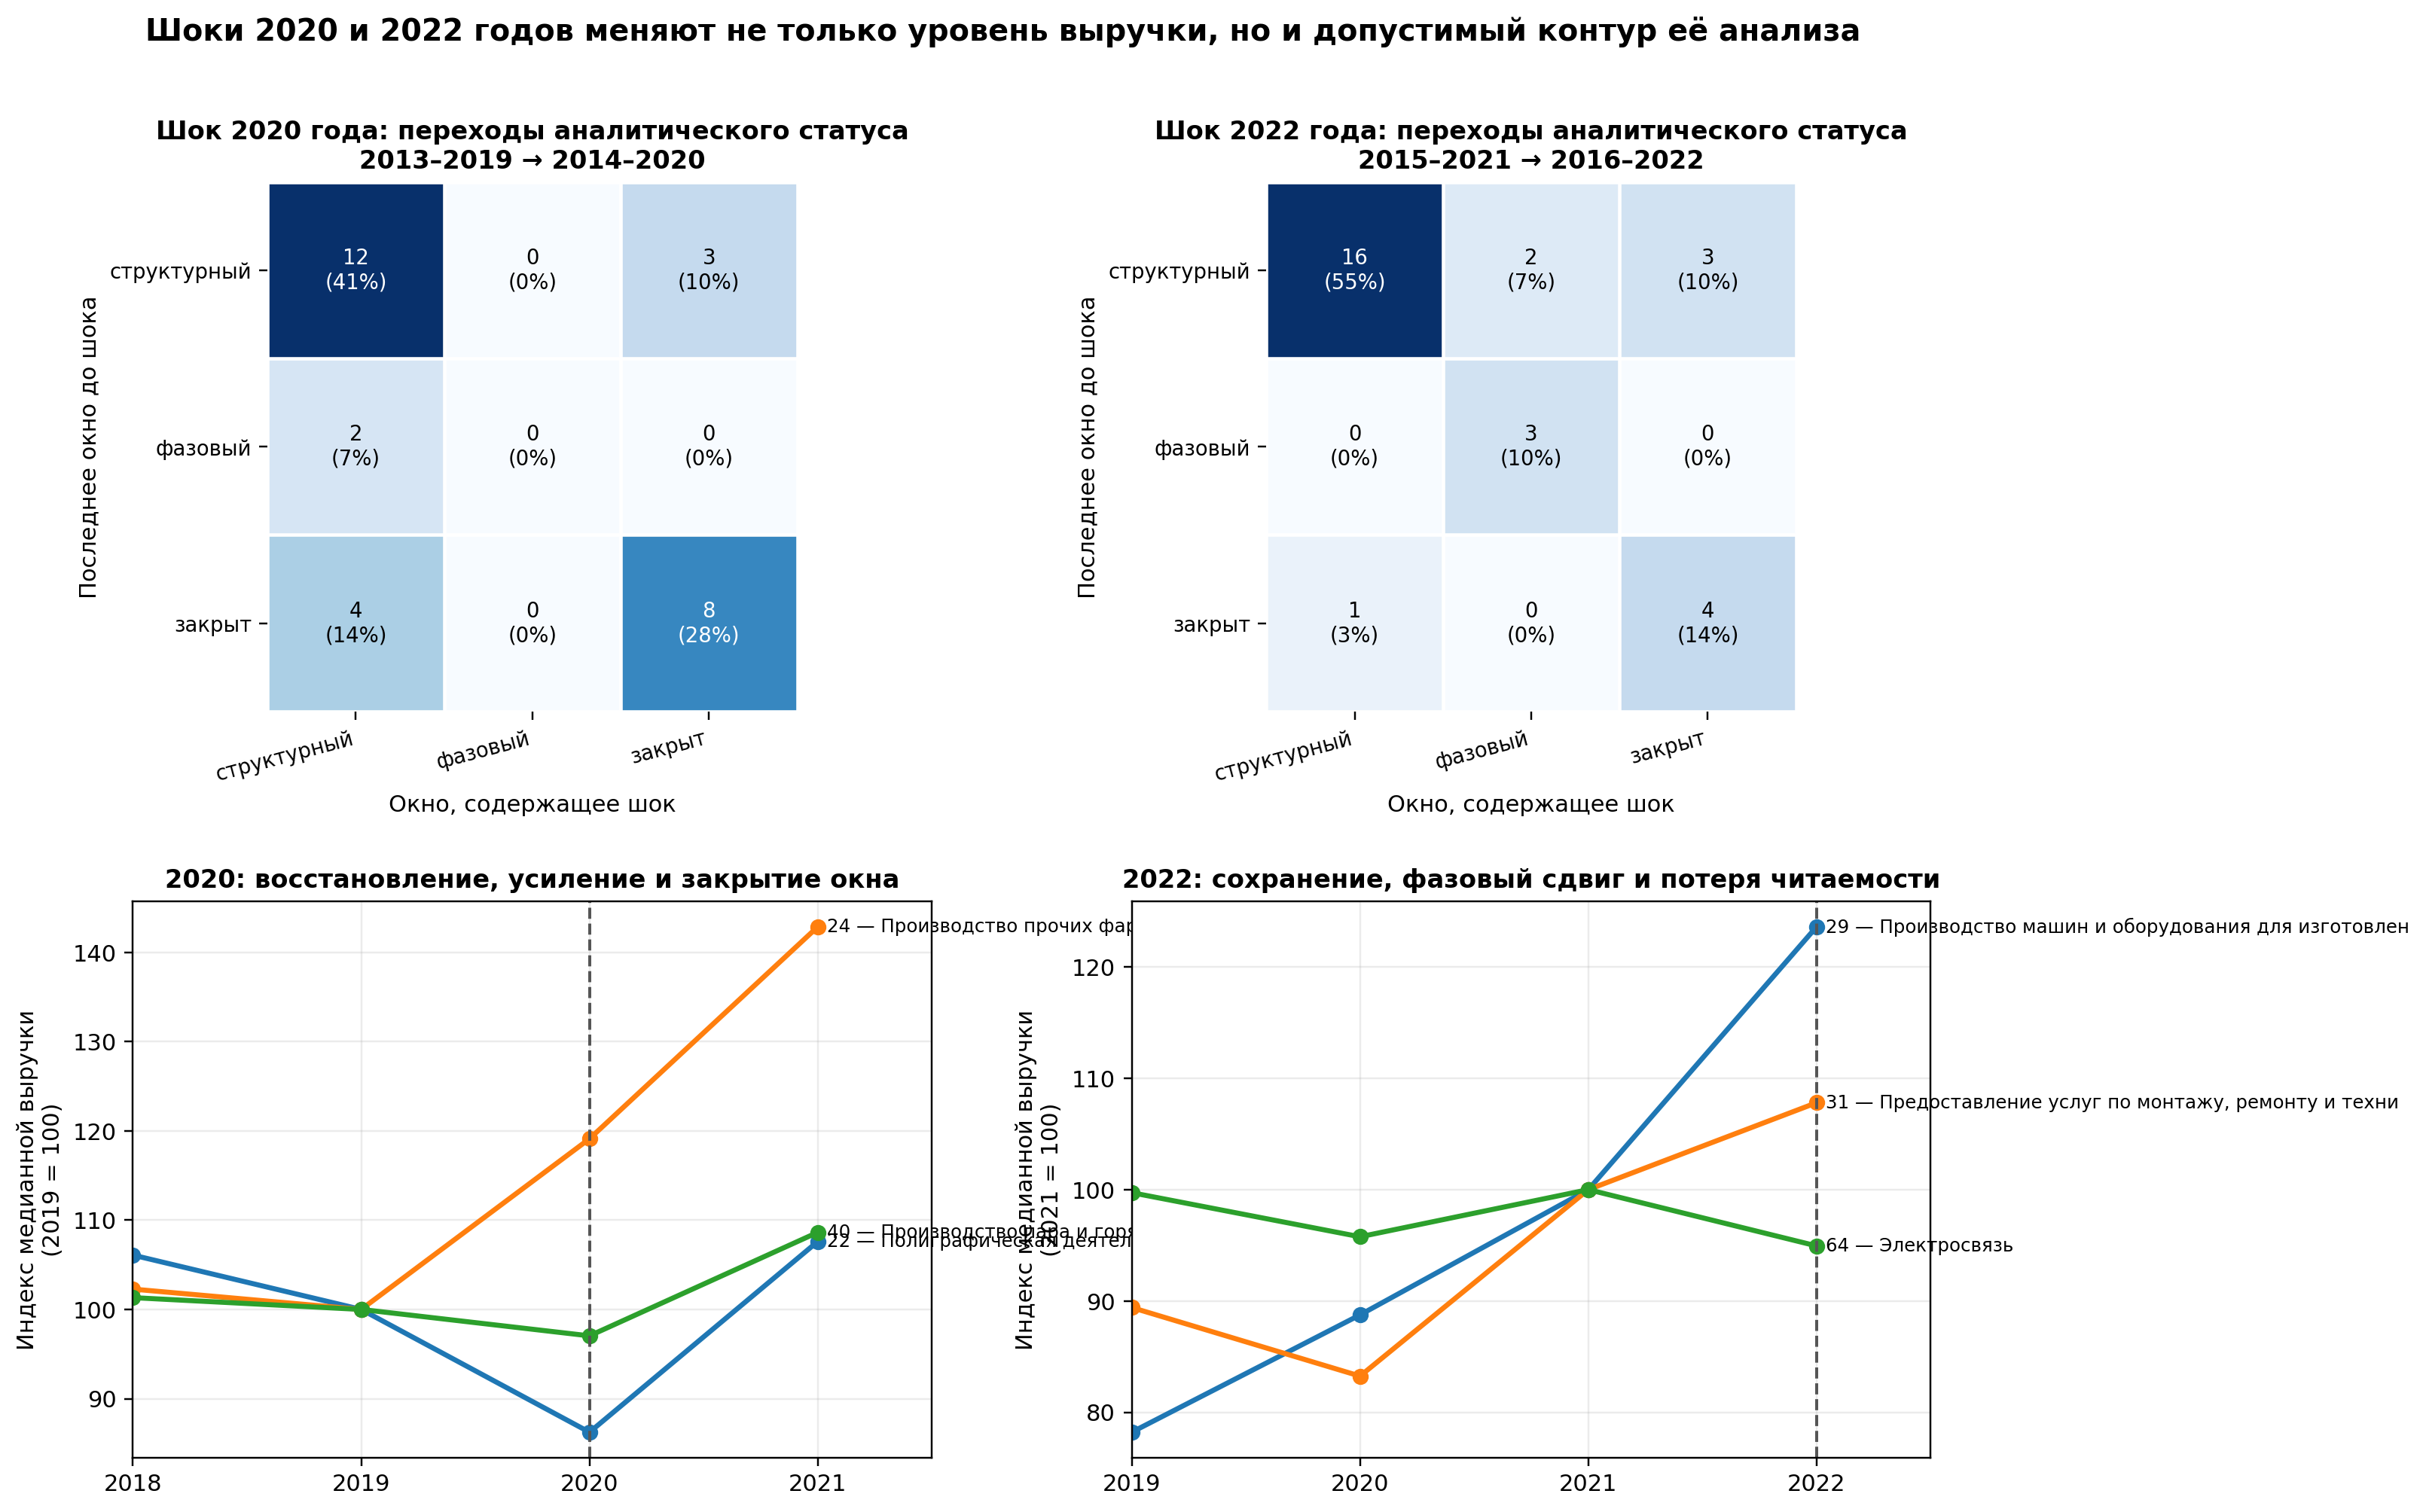
\includegraphics[width=0.98\textwidth]{../outputs/real_data/revenue_b2/shock_transition_map.png}
\caption{Шоки 2020 и 2022 годов как переходы аналитического статуса отраслевых рядов\\ \textit{Источник: расчёты автора по данным корпуса ``Данные по выручке 2003--2022.xlsx'' после отраслевой фильтрации.}}
\label{fig:shock-transition-map}
\end{figure}

Рисунок~\ref{fig:shock-transition-map} фиксирует главный результат этого блока. В 2020 году шок чаще открывал аналитически содержательное чтение, чем разрушал его: из 29 отраслей шесть улучшили свой статус и перешли к структурному контуру, тогда как три отрасли, напротив, утратили прежнюю читаемость. В 2022 году картина иная. Здесь уже преобладают неблагоприятные переходы: пять отраслей, ранее допускавших структурное чтение, переходят либо к фазовому контуру, либо в полностью закрытое состояние, тогда как улучшение наблюдается только в одном случае. Следовательно, 2020 год в отраслевом корпусе чаще выступает как шок с возможностью адаптации и возврата к содержательным окнам, тогда как 2022 год чаще сопровождается деградацией уже читаемого режима.

Нижние панели рисунка~\ref{fig:shock-transition-map} показывают, что этот результат не исчерпывается формальным перерасчётом меток. В 2020 году полиграфическая деятельность и выпуск фармацевтической продукции переходят от закрытого окна к структурно читаемому режиму; в обоих случаях шок не разрушает траекторию, а делает её более различимой. Иной тип реакции демонстрирует теплоснабжение: здесь шок не выглядит катастрофическим по уровню выручки, однако именно после него окно теряет содержательную структурную интерпретацию. Для 2022 года характерен другой набор примеров. Производство машин и оборудования для пищевой промышленности сохраняет структурный контур и после входа в шоковое окно. Монтаж и техническое обслуживание оборудования смещается в фазовый контур, то есть ряд остаётся читаемым, но уже требует иной процедуры анализа. Электросвязь, напротив, утрачивает содержательную интерпретируемость и переходит в закрытый режим.

Таким образом, шоковые годы в данном корпусе различаются не только направлением изменения выручки, но и тем, как они воздействуют на саму возможность анализа ряда. Этот вывод непосредственно продолжает аппарат главы~2: важен не только масштаб отклонения, но и то, переводит ли шок ряд в структурный, фазовый или закрытый режим. Именно поэтому 2020 и 2022 годы здесь интерпретируются не как две даты на графике, а как два разных теста на устойчивость аналитического контура.

\section{Прикладной алгоритм анализа короткого окна на реальных данных}
\label{sec:prikladnoi-algoritm-analiza-korotkogo-okna-na-realnyh-dannyh}

По результатам главы 3 прикладной алгоритм анализа короткого окна на реальных данных может быть записан в виде четырёх шагов.

\begin{enumerate}
\def\labelenumi{\arabic{enumi}.}
\tightlist
\item
  Сначала определяется режим траектории: монотонный, колебательный, шоковый или вырожденный.
\item
  Затем проверяется интерпретируемость окна: достаточно ли в нём сигнала, не вырождается ли оно по дисперсии и не схлопывается ли в коллинеарность.
\item
  После этого выбирается допустимый контур чтения: структурная регрессия, фазовое чтение или отказ от содержательной интерпретации.
\item
  Только на последнем шаге обсуждаются коэффициенты, знак памяти, шоковые переломы и прикладной смысл полученного окна.
\end{enumerate}

Именно этот маршрут и составляет основной перенос результата главы 2 на реальные данные: не универсальная модель, а процедура отбора допустимого способа анализа.

\section{Общие выводы по главе реальных данных и практическая значимость}
\label{sec:obschie-vyvody-po-glave-realnyh-dannyh-i-prakticheskaya-znachimost}

Итоги эмпирической части можно свести к таблице~\ref{tab:real-data-summary}.

\begin{center}
\captionof{table}{Сводные результаты эмпирической части}
\label{tab:real-data-summary}
\end{center}

{\def\LTcaptype{none} % do not increment counter
\begin{longtable}[]{@{}
  >{\raggedright\arraybackslash}p{(\linewidth - 8\tabcolsep) * \real{0.2000}}
  >{\raggedright\arraybackslash}p{(\linewidth - 8\tabcolsep) * \real{0.2000}}
  >{\raggedright\arraybackslash}p{(\linewidth - 8\tabcolsep) * \real{0.2000}}
  >{\raggedright\arraybackslash}p{(\linewidth - 8\tabcolsep) * \real{0.2000}}
  >{\raggedright\arraybackslash}p{(\linewidth - 8\tabcolsep) * \real{0.2000}}@{}}
\toprule\noalign{}
\begin{minipage}[b]{\linewidth}\raggedright
Корпус
\end{minipage} & \begin{minipage}[b]{\linewidth}\raggedright
Что удалось интерпретировать
\end{minipage} & \begin{minipage}[b]{\linewidth}\raggedright
Что не удалось интерпретировать
\end{minipage} & \begin{minipage}[b]{\linewidth}\raggedright
Почему
\end{minipage} & \begin{minipage}[b]{\linewidth}\raggedright
Практический вывод
\end{minipage} \\
\midrule\noalign{}
\endhead
\bottomrule\noalign{}
\endlastfoot
Промышленные индексы & переносимость режима анализа и выбор рабочего слоя наблюдения & устойчивую структурную интерпретацию всех отраслевых окон & часть окон вырождается или зависит от способа сглаживания & промышленный корпус пригоден как внешняя проверка метода \\
Группы компаний по выручке & различие между группами высоких, низких и средних темпов роста по допустимому контуру чтения & полные интервалы как готовую лаговую структуру & высокое качество подгонки часто сочетается с низкой локальной информативностью & анализ групп следует вести через короткие окна \\
Отраслевой подкорпус выручки & карту отраслевой читаемости и шоковые паттерны 2020 и 2022 годов & единый способ чтения для всех секторов & отрасли различаются по режиму и интерпретируемости окна & сектора нужно заранее разделять по допустимому аналитическому контуру \\
\end{longtable}
}

\subsection{Основные выводы главы}
\label{sec:osnovnye-vyvody-glavy}

В рамках проведённого исследования получены три основных результата.

\begin{enumerate}
\def\labelenumi{\arabic{enumi}.}
\tightlist
\item
  Перед запуском регрессии необходимо отбраковывать окна, не допускающие содержательной интерпретации.
\item
  Различение режима должно предшествовать выбору аналитического контура.
\item
  Работа с выручкой групп и отраслей требует коротких окон и предварительной проверки допустимости чтения, а не прямого использования полного интервала.
\end{enumerate}

Именно в этом состоит главный итог главы: реальные данные по выручке допускают содержательный анализ только после предварительной процедуры отбора и интерпретации окна.

\subsection{Практическая значимость}
\label{sec:prakticheskaya-znachimost}

Практическая ценность полученного результата состоит в трёх типовых применениях.

\begin{enumerate}
\def\labelenumi{\arabic{enumi}.}
\tightlist
\item
  Отбраковка неинтерпретируемых окон снижает риск ложных выводов по данным, где высокое качество подгонки создаёт лишь видимость устойчивой структуры.
\item
  Предварительное различение режимов позволяет выбирать метод анализа до запуска регрессии, а не после получения случайного набора коэффициентов.
\item
  Более аккуратная работа с выручкой групп и отраслей делает возможным содержательное сравнение траекторий без подмены интерпретации простым ранжированием по \(R^2\).
\end{enumerate}

Такой подход может быть полезен исследователю, отраслевому аналитику, макроаналитику и корпоративному аналитику в тех задачах, где приходится работать с короткими и режимно неоднородными рядами.

\subsection{Ограничения и итоговый вывод}
\label{sec:ogranicheniya-i-itogovyi-vyvod}

Полученные результаты не следует трактовать как универсальную прогностическую схему или как основание для прямого сравнения любых экономических рядов. В настоящей главе исследовалась прежде всего допустимость содержательного чтения короткого окна на реальных данных по выручке. Поэтому корректнее говорить не о единой модели для всех рядов, а о процедуре анализа, которая позволяет сначала определить режим, затем проверить интерпретируемость окна и только после этого переходить к коэффициентам и локальной структуре.

Итоговый вывод главы 3 состоит в следующем: режимно-зависимый подход, построенный в синтетической части, переносится на реальные данные по выручке как процедура отбора и допустимой интерпретации коротких окон. Его практический смысл состоит не в максимизации качества подгонки, а в снижении риска ошибочного чтения групповых и отраслевых денежных траекторий.
